\documentclass[a4paper,8pt]{article}
\usepackage{xcolor}
\usepackage{graphicx}
\usepackage{listings}
\usepackage{color}
\usepackage[T1]{fontenc}
\usepackage[polish]{babel}
\usepackage[utf8]{inputenc}

\definecolor{dkgreen}{rgb}{0,0.6,0}
\definecolor{gray}{rgb}{0.5,0.5,0.5}
\definecolor{mauve}{rgb}{0.58,0,0.82}

\lstset{frame=tb,
  language=Java,
  aboveskip=3mm,
  belowskip=3mm,
  showstringspaces=false,
  columns=flexible,
  basicstyle={\small\ttfamily},
  numbers=none,
  numberstyle=\tiny\color{gray},
  keywordstyle=\color{blue},
  commentstyle=\color{dkgreen},
  stringstyle=\color{mauve},
  breaklines=true,
  breakatwhitespace=true,
  tabsize=5
}
\graphicspath{ {./images} }

\begin{document}


\title{{\Large}Zadanie numeryczne 1}
\date{}
\author{Jakub Heczko}

\maketitle


\section{Opis uzytego algorytmu wraz z optymalizacja}


Algorytm jakiego uzylem jest algorytmem lekko skroconym od pierwotnej jego wersji, albowiem uzylem uproszczonego arytmetycznie wyrazenia, ktore wyglada nastepujaco:

\begin{center}
    $\frac{e^{3n}-e^{3n}cos(nx^4)^2+cos(nx^4)}{e^{4n}}$
\end{center}

Uzycie takiego wyrazenia sprawia, ze moge z praktycznie taka sama dokladnoscia wyliczac wartosci, ale o wiele szybciej, poniewaz licze wartosc cos() tylko raz, a nastepnie podstawiam pod odpowiednie miejsca w moim rownaniu, jesli chodzi o blad jaki jest miedzy dwiema wyrazeniami w sumach, to jest on taki sam, jesli porownamy go z prawdziwa wartoscia, wyliczona przez program wolframalpha:
\newline
\newline
\quad -Dla starego wyrazenia:
\newline
\newline
1.400781361326889\textcolor{red}{4074}
\newline
\newline
\quad -Dla nowego wyrazenia:
\newline
\newline
1.400781361326889\textcolor{red}{3018}
\newline
\newline
\quad -Dla wolframalpha:
\newline
\newline
1.400781361326889\textcolor{red}{3571}
\newline

Ze wzgledu na dlugosc wyniku w wolframie skrocnej dlugosc do takiej samej cyfry, jakiej dostalem wynik w moich wyrazeniach. Widzimy ze nasz blad dla jednego i drugiego wyrazenia jest bardzo zblizony, a zaoszczedza nam to obliczen. W tym "nowym wyrazeniu" niestety dalej bedziemy mieli do czynienia z bledem pochodzacym z odejmowania bliskich liczb od siebie, ale przynajmniej nie bedziemy musieli, wyliczac tej samej wartosci po kilka razy w kodzie. Drugim sposobem najbardziej optymalnym w pythonie, będzie uzycie sumy z biblioteki numpy, co zrobilem, tak jakby w dalszej czesci, programu, ale moją ilość operacji będe liczył dla tej pierwszej sumy, czyli recznie po kolei w petli for z uzyciem powyzszego wzoru.

\section{Uzasadnienie wyboru n}

Z wyborem n jest troche dwuznacznie, dlatego ze wybierajac n = 50 gwarantujemy maksymalnie dokladny wynik dla danego wyrazania przy uzyciu float64, ale na potrzeby zadania aby zminimalizowac ilosc obliczen, ale rowniez otrzymac blad mniejszy od $10^{-10}$ to najlepiej uzyc n = 23. Taki blad mowi nam, ze musimy miec co najmniej 8 cyfr znaczacych po przecinku, aby nasz blad nie przekroczyl podanej wartosci. 
\newline
Moj wybor wiec uzasadnie kilkoma rzeczami, po pierwsze danymi, ktore dostawalem; wygenerowalem okolo 20 roznych zestawow i dla kazdego, owy blad wynosil nawet mniej bo $10^{-12}$. Podam przyklad dla x = 15(oczywiscie jest to wynik sumy):
\quad -Dla programu:
\newline
\newline
1.42518273948\textcolor{red}{30521315}
\newline
\newline
\quad -Dla wolframalpha:
\newline
\newline
1.42518273948\textcolor{red}{89998731}
\newline
\newline
\quad -Wyliczylem blad i wynosi w przyblizeniu:
\newline
\newline
$9*10^{-12}$
\newline
Jak widac, nie jest tak zle, kiedy bedziemy porownywac wartosci z programu, z wartosciami z wolframa. Ale mam jeszcze drugi powod do wybierania takich n jak podalem powyzej, a jest to wykres funckji jakiej sume liczymy. Bardzo z gory przepraszam za jakos zdjecia mam nadzieje, ze bedzie na nim wszystko widac, ale wolfram nie pozwala mi w lepszej jakosci go wyeksportowac:
\newline
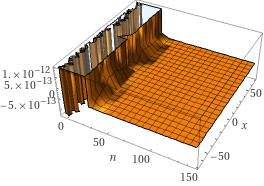
\includegraphics{wykres}
\newline
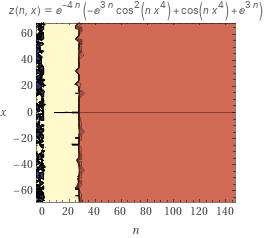
\includegraphics{mapa}
\newline
Pierwszy wykres, ukazuje sam wykres, a drugi jedynie mape poziomu skoku wykresu. Jak widac na wykresie wybranie dowolnego x nie zmieni nam, jak bedzie wygladac skladnik sumy dla n = 50, bo bedzie on bardzo zblizony do zera, ale jak mozna rowniez zauwazyc, ze nasze n dla okolo wartosci n = 20-25, wartosc tego elementu, ktory bedziemy dodawac do sumy bedzie bliska 0, co sprawi ze nasza suma sie nie zmieni, albo w bardzo malo znaczacy sposob. Lecz na wykresie pierwszym wydac, ze lekkie skoki sa nawet po n $\approx$ 25, lecz dopiera na n = 50 wszystko sie stabilizuje, co tlumaczy, dlaczego, nasza suma jest najbardziej dokladna dla n = 50.
\newline
Jest jeszcze trzeci argument za wyborem mojego n, jesli w mojej sumie przyjmiemy, ze cos(x) = 1, moge tak przyjac dlatego ze jest on ograniczony w zbiorze wartosci przez 1 z gory, wiec w zasadzie w nieskonczonosci nie powinno to nam jakos bardzo zmienic jak zachowuje sie ten ciag w nieskonczonosci. Wiec zapisuje moje rownanie bez cos(x), dostaje wiec:
\newline
\newline
\begin{center}
  $X_{n} = \frac{1}{e^{4n}}$
\end{center}
Teraz zapiszmy ogolne rownanie dla bledu tej sumy, czyli chcemy aby nasza suma do $+\infty$ - suma do jakiegos okreslone n byla mniejsza od $10^{-10}$. Daruje sobie wstawiania obliczen a jedynie sam wynik z wolframa.
\begin{center}
  $\mid S_{\infty} - S_{n}| \leq 10^{-10}$
  \newline
  \newline
  $\frac{1}{e^{4}-1}-\frac{1-e^{-4n}}{e^4-1} \leq 10^{-10}$
\end{center}
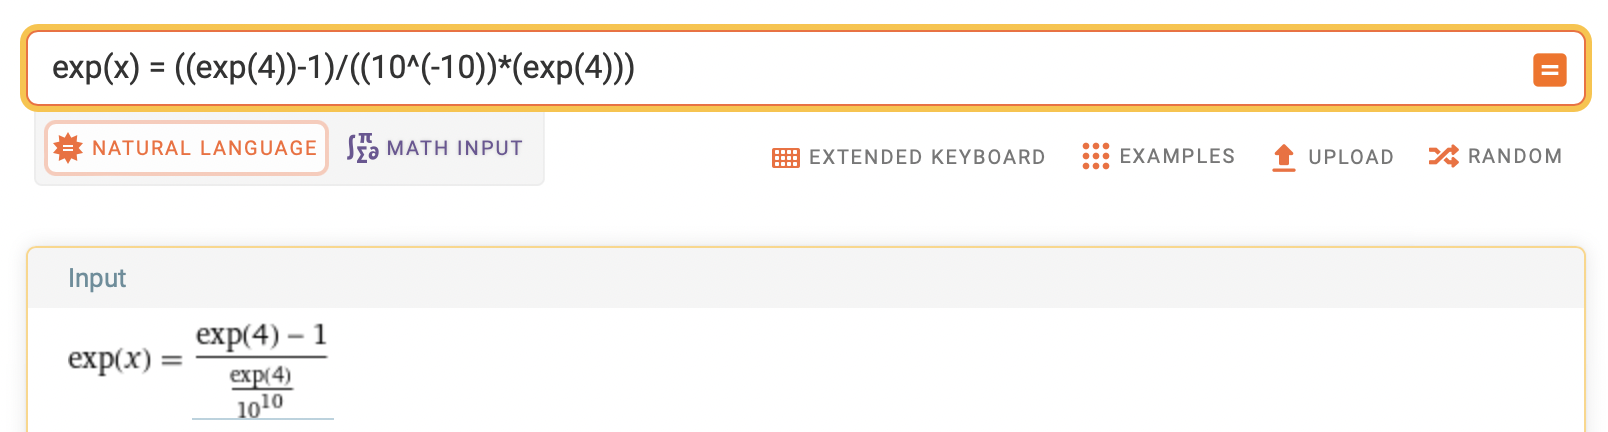
\includegraphics[width=10cm,height=10cm,keepaspectratio]{obliczenia1}
\newline
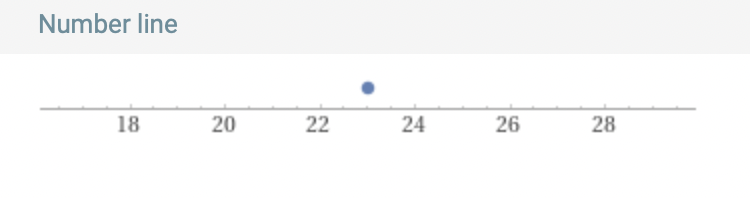
\includegraphics{obliczenia2}
\section{Polecenia do zadania}


\subsection*{Wartosc dla f(1)}
$f(1) = 1.4007813613$
\newline
$\epsilon = 0.0000000000002433608869978343 \newline lub \newline\epsilon = 2.433608869978343e-13$
\newpage
\subsection{Ilosc obliczen}
\begin{lstlisting}
(1)import exp from math
(2)import numpy as np
(3)def func(x):
(4)  value1 = np.longdouble(0.0)
(5)  for n in range(0,23):
(6)    cos_val = np.cos(n*(x**4))
(7)    value1 += np.longdouble( (exp(3*n) - exp(3*n)*cos_val*cos_val + cos_val) / exp(4*n))
\end{lstlisting}
To teraz linika po linice przelicze:
\begin{flushleft}
(1) 50 (parse)\textcolor{blue}{=50}
\newline
\newline
(2) 50 (parse)\textcolor{blue}{=50}
\newline
\newline
(3) 0.5(=) + 50(parse)\textcolor{blue}{=50.5}
\newline
\newline
(4) 50 (parse) + 0.5(=) + 1*23(warunek) + 1*23(+=) \textcolor{blue}{= 96.5}
\newline
\newline
(5) 0.5(=) + 30(cos) + 1*5(*) + 50(parse) to wszystko razy 23(petla) \textcolor{blue}{= 1966.5}
\newline
\newline
(6) 1(+=) + 3*30(exp, mamy 3 takie wywołania) 1*7(-/+/*/dzielenie) + 50(parse) to wszystko razy 23 \textcolor{blue}{= 3404}
\newline
\newline
(7) 50(parse)\textcolor{blue}{=50}
\newline
\newline

\textcolor{red}{Lacznie mamy operacji = 5667,5}
\end{flushleft}


\end{document}
